\textbf{Water heater object GLD Dec 19, 2020}
\subsection{objective}

    
    Test water heater behavior in GridLAB-D.
    
\subsection{outline}
    
    Using GridLAB-D, a water heater behavior is tested using the following parameter:
\subsection{procedures}
    
    To achieve the goal of this sprint, IEEE$\_$4$\_$Node$\_$Feeder is used. The following objects are needed:
    \begin{itemize}
        \item Triplex objects such as transformers, lines, meter, and water heater.
        \item Water heater parent. Typically a house object.
        \item Water heater object.
    \end{itemize}
    
\subsection{parameters}
    
    \begin{itemize}
        \item Setpoint 120F
        \item Deadband 2F
        \item Volume 50 Gallons
        \item Water demand ELCAP data
        \item heat$\_$mode ELECTRIC
    \end{itemize}
    
\subsection{Data}
    glm file can be found here \par  \url{https://github.com/psu-powerlab/GridLab-D/blob/master/NeoChargeProject/WH_4_Node_Feeder/Uncontrolled_WH/WH_4_node.glm}

    \par Full output data is uploaded to PSU power lab GitHub account, GridLAB-D repository.
    
    \url{https://github.com/MidrarAdham/GridLab-D/blob/master/NeoChargeProject/WH_4_Node_feeder/Water_heater/wh_1.csv}
\newpage
\subsection{results}
        \begin{figure}[hbt!]
            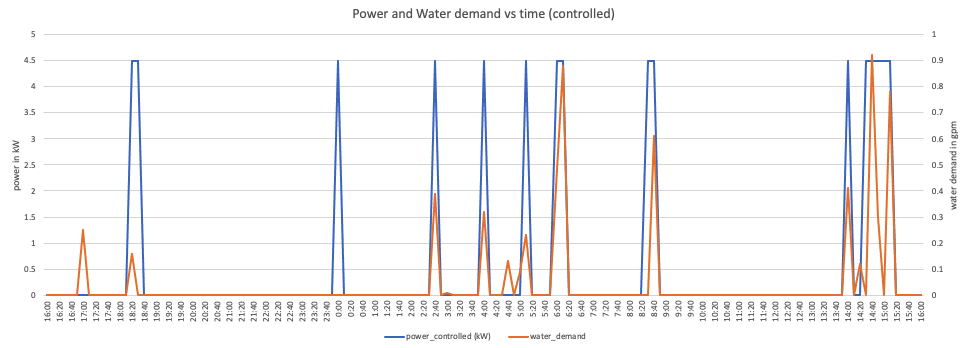
\includegraphics[scale=0.5]{Pictures/controlled_WH.png}
            \caption{Power and Water Demand vs Time (un-controlled)}
            \label{fig:uncontrolled_wh}
        \end{figure}

\newpage